\documentclass[report.tex]{subfiles}
\begin{document}

This first chapter presents the theoretical foundation for the thesis.
The theory is grouped into three sections: \glspl{NN}, learning and
neuromorphic hardware.\index{neuromorphic}

\section{Neural networks} \label{sec:nn}
\Glspl{NN} is a broad term that originates in the neuronal models from
the biological brain \cite{Dayan2001}.
The general architecture of neural systems can be explained as circuits
of neurons \index{neuron} connected through weighted edges
\cite{Russel2007, Dayan2001}.

In this abstract sense, a neuron is a computational unit that
takes a number of signals (inputs) and processes them through some
function $f$,that outputs a single value \cite{Eliasmith2004}.
Composed in a network, neurons can \textit{compute} 
complex non-linear functions \cite{Eliasmith2004, Dayan2001}.

In a more concrete sense, \gls{NN}s compute over either
continuous (e.g., voltage and numbers) or discrete signals
\cite{Russel2007, Schmidhuber2014}.
Discrete models were the foundation for
the first generation of neural networks \cite{Russel2007, Maass1997}.
They are based on the perceptron model as seen in Equation
\ref{eq:perceptron}, also known as the McCulluch-Pitts neuron model
\cite{Eliasmith2004}.

\begin{equation} \label{eq:perceptron}
\sigma(x) = \begin{cases}
	 1 & \text{if } x > 0\\
	 0 & \text{otherwise}
       \end{cases}
\end{equation}

\subsection{Neural networks as directed graphs} \label{sec:nn_graphs}
These first \glspl{NN} would collect neurons in groups\index{neuron!group} 
that connect to other groups in a sequence
\cite{Russel2007}.
Figure \ref{fig:nn-example} shows an example of such a network.
\begin{figure}
\centering
\tikzset{%
  every neuron/.style={
    circle, draw, minimum size=0.5cm
  },
  neuron dots/.style={
    draw=none,
    scale=1.5,
    text height=0.3cm,
    execute at begin node=\color{black}$\vdots$
  }
}
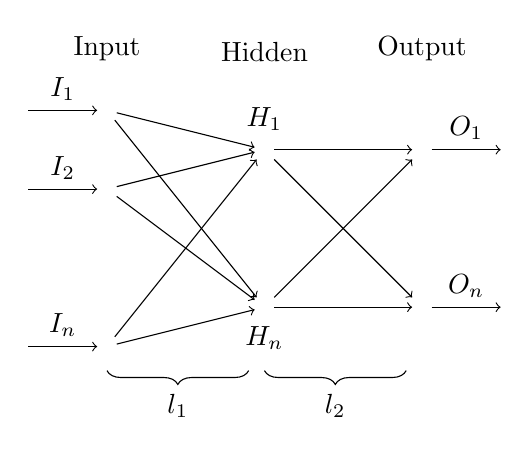
\begin{tikzpicture}{x=1.5cm, y=1.5cm}
  \foreach \m [count=\y] in {1,2,dots,n}
    \node [every neuron/.try, neuron \m/.try](input-\m) at (0, 2.5-\y) {};
  \foreach \m [count=\y] in {1, dots, n}
    \node [every neuron/.try, neuron \m/.try](hidden-\m) at (2, 2-\y) {};
  \foreach \m [count=\y] in {1, dots, n}
    \node [every neuron/.try, neuron \m/.try](output-\m) at (4, 2-\y) {};

  \foreach \l [count=\i] in {1, 2, n}
    \draw [<-] (input-\l) -- ++ (-1, 0)
      node [above, midway] {$I_{\l}$};
  \node [above] at (hidden-1.north) {$H_1$};
  \node [below] at (hidden-n.south) {$H_n$};

  \foreach \f in {1, 2, n}
    \foreach \t in {1, n}
      \draw [->] (input-\f) -- (hidden-\t);
  \foreach \f in {1, n}
    \foreach \t in {1, n}
      \draw [->] (hidden-\f) -- (output-\t);
  \foreach \l [count=\i] in {1,n}
    \draw [->] (output-\l) -- ++(1,0)
	node [above, midway] {$O_\l$};

  \foreach \l [count=\x from 0] in {Input, Hidden, Output}
    \node [align=center, above] at (\x*2,2) {\l};
  
  \draw [decorate,decoration={brace, amplitude=5pt,mirror,raise=4ex}]
    (0,-1.2) -- (1.8,-1.2) node[midway,yshift=-3em]{$l_1$};
  \draw [decorate,decoration={brace, amplitude=5pt,mirror,raise=4ex}]
    (2,-1.2) -- (3.8,-1.2) node[midway,yshift=-3em]{$l_2$};
\end{tikzpicture}
\caption{An example neural network of depth 3 with two layers ($l_1$, $l_2$) and a single hidden neuron group ($H$).}
\label{fig:nn-example}
\end{figure}

The number of groups determines the depth\index{neural network!depth} of
a network\cite{Russel2007}.
Each group applies a non-linear transformation to the input that is forwarded
to the next layer and so on \cite{Bishop2006, Russel2007}.
From a computational point of view a neuron group is simply a computational
unit, which allows \glspl{NN} to be abstracted as circuits of units connected in
a directed graph
\cite{Dayan2001, Eliasmith2004, Russel2007}.
This view can be simplified as shown in figure \ref{fig:nn-composition},
such that each neuron group\index{neuron!group} (node)\index{node}
is considered a function \cite{Rojas1996}.
Here the output is found by the sequential
composition of activation functions over the input $x$.
\begin{figure}
\centering
\tikzset{%
  node/.style={
    circle, draw, minimum size=0.8cm
  }
}
\begin{tikzpicture}
  \node (input) at (-0.3,0) { $x$ };
  \node [node] (node-f) at (1.5,0) { $g$ };
  \node [node] (node-g) at (3,0) { $h$ };
  \node (output) at (5,0) { $g(h(x))$ };
  \draw [->] (input) -- (node-f);
  \draw [->] (node-f) -- (node-g);
  \draw [->] (node-g) -- (output);
\end{tikzpicture}
\caption{Another representation of the network in Figure
  \ref{fig:nn-example}, where each layer is considered a function ($l_1 = g$, $l_2 = h$),
and the output is derived by composing functions sequentially 
over the input ($x$).}
\label{fig:nn-composition}
\end{figure}

Neuron groups are sometimes referred to as \textit{layers}\index{neural network!layer} \index{layer|see neural network}
in the literature, but from a computational perspective it is simpler to view layers as
functions, such that they include the output activations for the next neuron group \cite{Bishop2006}.
In this thesis, a layer is defined as computational units that transform input
with a non-linear function to produce some output.
Thus the network in figure \ref{fig:nn-example} consists of two layers.

The layered design is typical for first and second generation networks, but 
can be generalised to the third generation as well, despite their parallel
nature \cite{Eliasmith2015}. %TODO: Move to 3rd gen
Neuron groups or layers that are not directly connected to the input or output
of the network is traditionally denoted as `hidden'\index{layer!hidden} because it is only
stimulated indirectly \cite{Russel2007}.

In this representation the `input' is a vector, whose
length is equal to the number of input neurons in the first layer.
Conversely, the `output' is a vector whose length
is controlled by the number of output neurons in the network.
An \gls{NN} can then be understood as a function $f$ that 
maps an input vector to an output vector of arbitrary size
\cite{Russel2007}.

Neuron models typically enrich the
input signals ($x$) with a linear equation as shown in Equation \ref{eq:weightedoutput},
where $\sigma$ is the neuron function
\cite{Schmidhuber2014, Russel2007}. 
For a single neuron $x$, the output signal is calculated through a weight ($w$)
and a bias ($b$). 
Weights and biases allow the model to adapt the relative importance of each
input neuron by modifying their weights and biases, thus allowing the
model to \textit{train} to a given domain \cite{Schmidhuber2014, Russel2007}.

For each neuron $x$ in the layer $j$, the output $x_j$ can be calculated given the activation value,
weight and bias from the previous layer ($i$) (see Equation
\ref{eq:weightedoutput}).
Here $u_j$ is the weighted sum of the output from the previous layer $i$, before
applying the activation function $\sigma$.

\begin{equation} \label{eq:weightedoutput}
x_j = \sigma(u_j) = \sigma\left(\left[\sum_{i=1}^n w_{i,j} x_i\right] + b_j \right)
\end{equation}

\subsection{Second generation neural networks}
Second generation neural networks augment the perceptron model by
a) allowing continuous output values of a neuron and b) parametrising
the computation of the neuron by adding an \textit{activation function}
\index{activation function} that determines the output of the neuron
\cite{Maass1997}.
\textit{Sigmoidal} functions are commonly used for activation functions
because they resemble the perceptron step function while 
retaining continuity (see Figure \ref{fig:sigmoid})
\cite{Maass1997}.

\begin{figure}
\centering
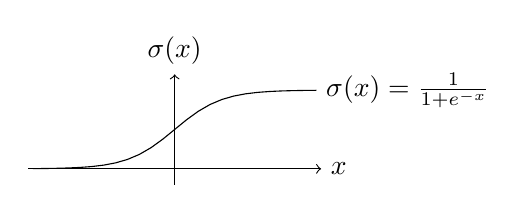
\begin{tikzpicture}[domain=-6:6,xscale=0.3]
  \draw[->] (-6.2,0) -- (6.2,0) node[right] {$x$};
  \draw[->] (0,-0.2) -- (0,1.2) node[above] {$\sigma(x)$};
  \draw plot (\x,{1 / (1 + exp(-\x))}) node[right] {$\sigma(x) = {1 \over 1 + e^{-x}}$};
\end{tikzpicture}
\caption{A sigmoidal (soft step) function.}
\label{fig:sigmoid}
\end{figure}

A number of variations for sigmoidal activation functions exist such as the 
hyperbolic tangent ($tanh$) and
the rectified linear unit \index{activation!ReLU} (ReLU, see Equation \ref{eq:ReLU}). 

They are applied either in a feed-forward or recurrent (cyclic) manner, where
the recurrent variant performs temporal transformations
\footnote{It is possible to \textit{unfold} recurrent
networks to resemble the circular processes until a certain point, achieving
a similar effect to temporal signal transformation, see \cite{Mozer1995}.}
\cite{Schmidhuber2014}.

\begin{equation} \label{eq:ReLU}
f(x) = \begin{cases}
         0 & \text{if } x < 0 \\
	 x & \text{otherwise}
       \end{cases}
\end{equation}

\subsubsection{Normalisation}
\index{normalisation}
To align with the activation output domain ($[0, 1]$), the input data
is typically normalised \cite{Bishop2006}.
One naïve approach is to divide by the maximum value of the input, but
that produces a linear effect, which is undesirable for reasons that will be
discussed later.
Instead, a sigmoidal function is typically used, because of its abovementioned
qualities.
One common variant for normalisation is the softmax\index{normalisation!softmax}
function, defined below given the input vector $x$ with $N$ elements:

\begin{equation}
  \sigma(x) = { e^x \over \sum^N_{n=1} e^x}
  \label{eq:softmax}
\end{equation}

\subsection{Third generation neural networks}
Constructing a network of neuron models essentially creates a non-linear
response to a given numerical vector \cite{Russel2007}.
This transformative view can be adopted to biological (third generation)
\glspl{SNN}, where the data being transferred are no longer vectors, but 
\textit{spikes}\index{neuron!spike}
of electrical current over time \cite[p. 32]{Dayan2001, Eliasmith2004}.

In biological networks there is a temporal dimension, in that neurons
produce and fire spikes asynchronously to other neurons in the same
group \cite{Eliasmith2004}.

Lapicque worked on a conductance model in 1907 that could describe this
process dubbed the \textit{integrate-and-fire} \index{neuron model!integrate-and-fire}
\index{integrate-and-fire|see {neuron model}}
model.
The model essentially integrates received current over time, and
if the integrated current reaches a certain threshold $V_{thr}$, the neuron
fires \cite{Dayan2001, Eliasmith2004}.
In biological neurons this also implies a spatial dimension, because the
current is sent through a neurons that extend in space \cite{Dayan2001}.
The cell body (soma)\index{neuron!soma} receives impulses from a number
of dendrites\index{neuron!dendrite}, and emits spikes through an 
axon\index{neuron!axon} \cite{Dayan2001}.
The geometry of the components influence the time as well as the amount of current
it requires to send impulses through the neuron \cite{Eliasmith2004}.
This has been modelled to a high degree of precision in the 
Hudgkin-Huxley model \cite{Dayan2001}.
While it is more precise than models below, it is
more complex \cite[p. 195]{Dayan2001} and rarely used in simulations
\cite{Albada2018, Dayan2001, Eliasmith2015}.

An idealised version of this is given in he Dirac ($\delta$) function \index{Dirac function}
in Equation \ref{eq:dirac} \cite[p. 404]{Dayan2001}.
For all values it approaches 0, except when its argument is
0 where it will grow infinitely.
In a trial starting at time $0$ and ending at time $t$, this
is the equivalent of summing up the $n$ neuronal events that occurred in 
the duration of the trial.
The total area of these `spikes' sum together to 1 over time $t$. \index{neuron spike}

\begin{equation} \label{eq:dirac}
  \rho(t) = \int_0^T \delta(t) = \sum_{i=1}^n \delta(t - t_i) = 1
\end{equation}

This idealised representation is a common mathematical approximation of
a sequence of activation functions \cite{Dayan2001, Eliasmith2004},
and the foundation for the \textit{third} generation
neural networks, where the computational unit is discrete events over time,
instead of continuous-valued (as in second generation \glspl{NN})
\cite{Maass1997}.\index{neuron spike}\index{spike|see {neuron spike}}

The spiking model is based on a neuron that builds voltage over time, until
it reaches a threshold voltage ($V_{th}$) and emits a spike
\mbox{($\delta(t-t_n)$)}
\cite{Dayan2001, Eliasmith2004}.
The spike carries a charge and is received by a post-synaptic neuron as
input current, which, in turn, decides whether to fire \cite{Dayan2001}.

After spiking the voltage inside the neuron is reset to a value ($\tau_{reset}$),
from which it begins to accumulate charge again.
In a brief period after the activation the neuron enters a period of
refraction, \index{refractory period}
where injected voltage is not accumulated, denoted by 
$\tau_{ref}$, illustrated in Figure \ref{fig:spiking}
\cite[p. 82]{Eliasmith2004}.

\begin{figure}
\centering

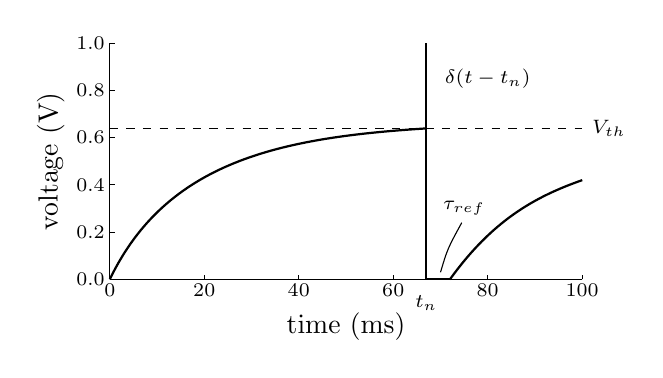
\begin{tikzpicture}[scale=3]
\pgfkeys{/pgf/number format/precision=1}
\draw (0,0) -- (2, 0);
\draw (0,0) -- (0, 1);
\foreach \i in {0,0.2,...,1}
  \draw (0,\i) -- (0.02,\i) node [left] {\scriptsize \pgfmathroundtozerofill{\i}\pgfmathresult};
\foreach \i in {0,20,...,100}
  \draw (\i/50,0) -- (\i/50,0.02) node [below] {\scriptsize \i};

\node [rotate=90] at (-0.25, 0.5) {\text{voltage (V)}};
\node at (1, -0.2) {\text{time (ms)}};

\draw [thick] (0,0) .. controls (12/50,0.50) and (36/50,0.6) .. (67/50, 0.639);
\draw [thick] (67/50,0) -- (67/50,1);
\draw [dashed] (0,0.64) -- (2,0.64) node [right] {\scriptsize $V_{th}$};
\node at (67/50, -0.1) {\scriptsize $t_n$};
\draw [thick] (67/50,0) -- ++ (0.1,0);
\node at (80/50,0.85) {\scriptsize $\delta(t-t_n)$};
\draw [thick] (72/50,0) .. controls (81/50,0.25) and (90/50,0.35) .. (2, 0.42);
\node at (75/50,0.3) {\scriptsize $\tau_{ref}$};
\draw (70/50,0.03) .. controls (71.5/50,0.13) .. (74.5/50,0.24);

\end{tikzpicture}
\caption{A model of how a constant, low input current produces a buildup of
	voltage inside a integrate-and-fire neuron, which eventually produces a spike.
	\index{neuron model!integrate-and-fire} 
	After spiking the neuron enters a refractory period, $\tau_{ref}$,
   	where no voltage is integrated.}
\label{fig:spiking}
\end{figure}

Lapicque's model has been elaborated in the \textit{leaky
integrate-and-fire} (LIF) \index{neuron model!leaky-integrate-and-fire}
model, which introduces a numerical ``leak''
into the model, that acts as a type of memory \index{memory}
for the neuron integration \cite{Eliasmith2004, Eliasmith2015}.
In the leaky model, input voltages decays exponentially over time,
meaning that the present voltage depends more strongly on recent input
voltages \cite[p. 85]{Eliasmith2004}.

\begin{equation}
  \frac{dv}{dt} = - {1 \over \tau_{RC}} (v - cr)
  \label{eq:lif}
\end{equation}

The LIF equation is given in Equation \ref{eq:lif}, where
$v$ is the membrane voltage difference between the interior
and exterior of the neuron membrane, $c$ is the input current, $r$
is the ionic current (or leak) of charge across the membrane, and
$\tau_{RC}$ is the membrane time constant that determines how
quickly the neuron decays to its resting state \cite{Dayan2001, Eliasmith2004}.
As the voltage builds up inside the neuron, $r$ will scale the
rate of growth \cite{Eliasmith2004}.
By tuning the leak it is possible to control the time with which
previous voltages are 'forgotten' \cite{Eliasmith2004}.

Similar to second generation neural networks, neurons
receive input from $n$ input neurons.
The connections are commonly referred to as synapses, and are similarly
weighted, as well as translated by a bias (see Equation \ref{eq:weightedoutput}),
such that they contribute differently to the accumulated 
voltage, given by Equation \ref{eq:synaptic} \cite{Dayan2001}.

\begin{equation}
  x_j = \sigma(u_j) = \sum_{i=1}^n{w_i\delta(t - t_i)} + b_j
  \label{eq:synaptic}
\end{equation}

\subsection{Coding spikes} \label{sec:coding}
Spikes convey information in the form of amplitude, duration, and
inter-spike intervals \cite{Dayan2001}.
A number of methods exist to decode the information in the spikes, by a 
combination of the three parameters \cite{Dayan2001, Eliasmith2015, Diehl2015, Rueckauer2017},
but this thesis will
focus on so-called rate models\index{rate encoding|see {encoding}}\index{encoding!rate}.
Recording neuron spikes over time provides an array of timestamps called a
spike train\index{spike train} \cite{Eliasmith2015}.
Rate models simply count the timestamps and divide them by the duration of
the trial to produce the spike \textit{rate}, shown
in Equation \ref{eq:spikerate} \cite{Dayan2001, Eliasmith2004}.
Semantically this is the equivalent of averaging the number of spikes propagated
in that interval, and provides the basis for a numerical interpretation of a
neuron's output \cite{Eliasmith2004}.

\begin{equation}
  r = {n \over T} = {n \over \rho(t)} = {1 \over T} \int_0^T \delta(t)
\label{eq:spikerate}
\end{equation}

When encoding numerical information to spikes, it is useful to 
express the spikes stochastically, such that one scalar determines
the probability that a neuron spikes over time \cite{Dayan2001}.
Assuming that the spikes are independent from each other, this
probability can be expressed by a probability distribution such as the
Poisson distribution\index{Poisson distribution}
\cite{Dayan2001}.
The Poisson distribution determines the probability of a number
of events occurring in an interval, given that the events are
known to happen at a fixed rate \cite{Dayan2001}.
It is defined in Equation \ref{eq:poisson} where $n$ is the
number of events and $\lambda$ is the rate with which events
happen \cite{Dayan2001}.
Figure \ref{fig:poisson} shows the probability that the number of
observed events ($k$) matches the poisson rate ($\lambda$).

\begin{equation}
P(n) = \lambda^n {e^{-\lambda} \over n!}
\label{eq:poisson}
\end{equation}

\begin{figure}
\centering
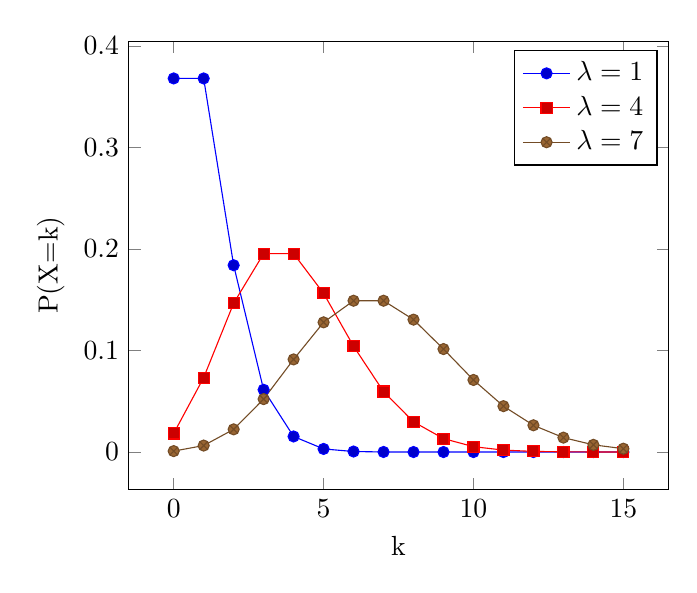
\begin{tikzpicture}
\pgfmathdeclarefunction{poiss}{1}{%
  \pgfmathparse{(#1^x)*exp(-#1)/(x!)}%
}
\begin{axis}[ylabel={P(X=k)},xlabel={k},legend
    entries={$\lambda=1$,$\lambda=4$,$\lambda=7$},every axis plot post/.append style={
    samples at = {0,...,15},
    axis x line*=bottom,
    axis y line*=left,
    enlargelimits=upper}]
  \addplot +[sharp plot] {poiss(1)};
  \addplot +[sharp plot] {poiss(4)};
  \addplot +[sharp plot] {poiss(7)};
\end{axis}
\end{tikzpicture}
\caption{The probability of a number of events ($k$) occurring, given the
poisson rates ($\lambda$) of 1 (blue), 4 (red) and 7 (brown).}
\label{fig:poisson}
\end{figure}

To align digital representations with neural spikes,
signals are encoded and decoded when entering and leaving the \gls{SNN}
\cite{Dayan2001}.
To compare between non-spiking and spiking networks is it necessary to 
provide a coding scheme that transfers between the two representations.

During the following, it is assumed that the input represents a constant
input current, and that the spike propagation follows the distribution
above.
The full proof is available in Appendix \ref{app:transfer}.

The argument goes as follows.
When simulating a LIF\index{neuron model!leaky-integrate-and-fire}
neuron at time $t$, the firing rate depends on the neuron firing threshold $V_{thr}$,
some input current $v(t)$, a maximum
firing rate $r_{max}$, and an activation of the input, following the
ReLU\index{activation!ReLU} activation function (Equation \ref{eq:relu}) and 
the linear scaling function in Equation \ref{eq:weightedoutput}:

\begin{equation}
x_i^l = max\left(0, \sum^{N^{l - 1}}_j= W^l_{ji} x_j^{l - 1} + b_i^j\right)
  \label{eq:relu_activation}
\end{equation}

The output is injected as current into the neuron, who will fire if the
potential exceeds the threshold.
Any surplus charge $\epsilon$ is discarded when the neuron is reset
after a spike, and will downscale the firing rate.
The spiking rate for a neuron $i$ at time $t$ in the first layer can
now be defined as:

\begin{equation}
r_i^1(t) = x_i^1 r_{max} {V_{thr} \over V_{thr} + \epsilon_i^1 } - {v_i^1(t) \over t (V_{thr} + \epsilon_i^1) }
\label{eq:spike_conversion}
\end{equation}

When the input and simulation time step is small the surplus
error $\epsilon$ goes towards 0, and can be ignored \cite{Rueckauer2017}.
For large simulations over long periods of time, however, the assumption
this has proven to be an issue for \citeauthor{Diehl2015} and
\citeauthor{Rueckauer2017}.
But for minor networks Equation \ref{eq:spike_conversion} shows a 
linear relationship between the spike rate and the input
\cite{Rueckauer2017}.
Because of the assumption that the constant input currents propagate as poisson rates
through the network, the networks and biases within the network will similarly
have to scale.

Transferring normalised input from \gls{ANN} to \gls{SNN}, then, is
a question of determining the exact scaling factor between the \gls{ANN} input
and the \gls{SNN} spiking rate.

\section{Learning} \index{learning} \label{sec:learning}
% TODO: http://www.cs.toronto.edu/~fritz/absps/momentum.pdf
Defining an \gls{agent} as a system that can act on previous knowledge
\cite{Russel2007}, learning in the context of an \gls{agent}
refers to ``the process of gaining
information through observation'' \cite{sep:learning-formal}.

Following the above abstraction of neural networks as computations over vectors,
``learning'' \index{learning} can be understood as the development of consistent
patterns, given the same input.
Within the \gls{ml} literature, this is commonly referred to as 
\textit{prediction}. \index{learning!prediction}
In practice this is expressed in terms of general functions or
\textit{rules} \index{rule} in a network \cite[p. 704.]{Russel2007}.

Within \gls{ml} systems are typically classified into
supervised, \index{learning!supervised}
unsupervised \index{learning!unsupervised} and reinforced learning systems.
\index{learning!reinforcement}

\textit{Supervised} learning relies on a set of expected outputs which 
the learning \gls{agent} must predict, given some input \cite{Russel2007}.
The \gls{agent} is told how `wrong' it was, so it can adapt accordingly.
Learning typically happens in a \textit{training} 
phase, where the \gls{agent} is allowed to build its internal representation 
\cite{Russel2007}.
This representation is later tested in the \textit{testing} phase, 
where the model is asked to infer based on previously unseen data \cite{Russel2007}.

\textit{Unsupervised} learning asks the \gls{agent} to learn without
having any idea of error margin \cite{Russel2007}.
Rather, the \gls{agent} is asked to \textit{explore} a domain in search of
patterns, which then form the basis for future predictions or classifications
\cite{Russel2007}.

\textit{Reinforced} learning reinforces the \gls{agent} through
rewards and discourages it through punishments \cite{Russel2007}.
Contrary to supervised learning the rewards and punishments are not
instructing the agent on what the output should be, but rather how well
it performed the task, leaving the \gls{agent} to infer rules or
behaviours by itself \cite[p. 873]{Russel2007}.

The process of learning can either be \textit{inductive}
\index{learning!induction}
or \textit{deductive} \index{learning!deduction} \cite[p. 704]{Russel2007}.
The latter requires a basis in rule-based systems from which new knowledge can
be deduced, while the former requires a measurement of success \cite[p. 705]{Russel2007}.
Such a measurement is typically referred to as the \textit{error} or \textit{loss}
function,\index{loss function}\index{error function|see {error function}}
because it shows how much the prediction deviated from the expectation (goal)
\cite{Russel2007}.

Learning within neural networks have shown to be possible within all three
types of learning \cite{Schmidhuber2014, Russel2007}, but deduction is rarely
seen in the literature, because it is cumbersome to express neural
networks through logic transformations \cite{Pearl2018}.

Because of its simplicity and widespread use, this thesis will focus on supervised
inductive learning.

\subsection{Errors in learning}
It is worth noting that \gls{NN}s may learn \index{learn}
rules \index{learning!rule} that are not optimal \cite{Russel2007}.
This can happen in one of two ways: either the
network is structurally incapable of learning the domain, 
or the learned rule is incorrect \cite{Russel2007, Eliasmith2015}.

A \gls{NN} is limited in complexity by its number of nodes,
since one neuron is expressed through its activation function
\cite{Dayan2001, Russel2007}.
Such a structural limit cannot be solved by any other means
than augmenting the network \cite{Russel2007}.

Seeing neural networks as complex non-linear systems, with
a number of parameters for the weights and biases,
the network can be visualised as a point in a high-dimensional space 
\cite{Russel2007}. 
Provided that the network is sufficiently complex, the 
learned rules can still fail to achieve a good accuracy because
the system falls into local minima \cite{Russel2007}.

A similar problem occurs when the model only trains on data
that is not representable for the more general domain \cite{Russel2007}.
This type of ``overfitting'' can be avoided by exploiting the 
training and testing phases from above, where networks
only train on \textit{parts} of the available data
\cite{Russel2007, Schmidhuber2014}.
The remaining data is applied in the testing phase to
validate the generalisation of the model.
The limits between data for training and data for testing
are not agreed upon, but a 80\% training/20\% testing split seems to be
the default \cite{Russel2007, Schmidhuber2014}.

\subsection{Backpropagation}
In the search for optimal weight/bias configurations,
such that prediction errors are minimised \cite{Rumelhart1988},
the network weights constitutes the search space, 
and the loss function \index{loss function}
is the subject of the optimisation \cite{Russel2007}.

One loss function to minimize for a supervised network
is described in Equation \ref{eq:bp-loss},
where the actual output $x$ is compared to the 
target (desired) output $t$, for all $n$ output neurons
\cite{Russel2007}.

\begin{equation}
  E = {1 \over 2} \sum_{i=1}^n |x_i - t_i|^2
  \label{eq:bp-loss}
\end{equation}

As has been shown, feedforward networks perform this calculation
through the sequential application of the weighted activation
functions in each layer.
One method to minimising this error is
to calculate the gradients of the network layers and iteratively walk in
the opposite direction of the error, a technique called gradient
descent \index{gradient descent}\cite{Rumelhart1988, Russel2007}.
Gradient descent requires that the network
activation functions are differentiable,
such that the gradient of $E$ with respect to the layer weights
($w_1 \cdots w_l$) can be found, and be iteratively
adjusted \cite{Rojas1996}, as shown in equation \ref{eq:bp-weights}.
Figure \ref{fig:ann_weights} visualises how the weights relate
to the output in a single-layer network.

\begin{equation}
  \Delta E = (
    {\partial E \over \partial w_1}, 
    {\partial E \over \partial w_2},
    \cdots, 
    {\partial E \over \partial w_l}
  )
  \label{eq:bp-weights}
\end{equation}

\begin{figure}
  \centering
  \includegraphics[width=0.6\textwidth]{images/ann.png}
  \caption{A visualisation of weights and biases in a single-layered neural
  network, given the input $x$ and output $y$ \cite{Mcstrother}.}
  \label{fig:ann_weights}
\end{figure}

Deriving the error function from Equation \ref{eq:bp-loss} gives

\begin{equation}
  \delta_j = y_j - t_j
  \label{eq:bp-loss-prime}
\end{equation}

The derivation of $E_n$ for an output neuron $n$ from layer $i$ to layer $j$
depends on the weight $w_{ji}$ via the activation input $u_j$ (see equation
\ref{eq:weightedoutput}).
The chain rule for partial derivations can now be applied \cite{Bishop2006}:

\begin{equation}
  {\partial E_n \over \partial w_{ji} } =
  { \partial E_n \over \partial u_j}
  {\partial u_j \over \partial w_{ji}}
  \label{eq:bp-chain}
\end{equation}

and replace the following terms

\begin{equation}
  \delta_j = 
  { \partial E_n \over \partial u_j}
  \qquad
  z_i = { \partial u_j \over \partial w_{ji}}
  \label{eq:bp-d}
\end{equation}

to get 
\begin{equation}
  {\partial E_n \over \partial w_{ji} } =
  { \partial E_n \over \partial u_j}
  {\partial u_j \over \partial w_{ji}} = 
  \delta_j z_i
  \label{eq:bp-chain2}
\end{equation}

Observing that $\delta_j$ can be further expanded to the sum of all units $k$
that receives input from unit $j$ such that

\begin{equation}
  \delta_j = {\partial E_n \over \partial u_j} =
  \sum_k {\partial E_n \over \partial u_k} 
  {\partial u_k \over \partial u_j}
  \label{eq:bp-d2}
\end{equation}
\noindent
and substituting Equation \ref{eq:bp-d} into Equation \ref{eq:bp-d2} while applying the chain rule, such that

\begin{equation}
  \begin{split}
  \delta_j & = \sum_k {\partial E_n \over \partial u_k} 
   {\partial u_k \over \partial u_j} \\
   & = \sum_k \delta_k {\partial u_k \over \partial \sigma_j} {\partial \sigma_j \over \partial u_k} \\
   & = \sum_k \delta_k w_{kj} \sigma'_j \\
   & = \sigma'_j \sum_k w_{kj} \delta_k 
  \end{split}
  \label{eq:bp}
\end{equation}

This more general form of backpropagation can be chained through layers, where
the outer most $\delta_j$ term---also called the layer ``error''---is defined 
as in Equation \ref{eq:bp-loss-prime}.

In each layer weights are updated as shown in equation \ref{eq:bp-update},
to approach an optimal configuration.
For biases, the derivative $\partial a_j \mathbin{/} \partial b_j = 1$ such that bias
updates are given by Equation \ref{eq:bp-update-bias}.
Here $\gamma$ is a factor that controls the speed with which the weights
are corrected (learning rate). \index{learning rate}

\begin{equation}
  \Delta w_i = -\gamma {\partial E \over \partial w_i}
  \label{eq:bp-update}
\end{equation}

\begin{equation}
  \Delta b_i = -\gamma \delta_j
  \label{eq:bp-update-bias}
\end{equation}

The learning rate exists to avoid ``shooting over'' optimal points
\cite{Russel2007}.
Typically a momentum is added to the learning rate, depending on the norm of
$\delta_j$, to scale the adaptation to the degree of error,
see \cite{Sutskever2013, LeCun1998}. 
Several other techniques have been invented to circumvent the problem of 
local minima and optimise the learning of the model \cite{LeCun1998,
Schmidhuber2014}, but they will not be covered here.

\subsection{Weight and bias normalisation}
When applying backpropagation in \gls{SNN} it is important to be aware of the dissonance
between the gradient, differentiable activation models and the LIF models
\cite{Diehl2015, Rueckauer2017}.
The approximated coding scheme from Section \ref{sec:coding} assists in the translation
of the input, but it is reasonable to normalise the weights and biases to avoid vanishing gradients.
\textcite{Rueckauer2017} proposed a scheme where weights are scaled according to the activation
potential of the previous layer, over the activation potential $a$ over the current layer:

\begin{equation}
w^l \rightarrow w^l {a^{l - 1} \over a^l}
\label{eq:weight_norm}
\end{equation}

Unfortunately this model is prone to outliers, and they propose a robust normalisation scheme,
where $a$ is set to a percentile of the activation values of a layer \cite{Rueckauer2017}.

\section{Neuromorphic computing}
Neuromorphic hardware is based on the idea of \gls{NN}s where the activation
units are modelled outside the classical \gls{vonNeumann}, either in 
integrated circuits or in simulated environments \cite{Albada2018,Blundell2018,Schmitt2017}.

This approach permits the simulators to work several hundred of magnitudes
faster than regular \gls{ANN}s, but at the cost of precision and noise
\cite{Indiveri2015, Schmitt2017}.
The precision problems occur because of hardware limitations where the typical
weight is restricted to a few bits, compared to larger \gls{ANN} networks
\cite{Indiveri2015, Lin2018}.
The noise problems are caused by noise in the integrated circuit components 
\cite{Lin2018, Pfeil2013}.

The technology is still relatively young and suffers from a number
of practical problems, why networks above a couple of thousand neurons remains
problematic in the available platforms \cite{Schmitt2017}.

The state-of-the-art neuromorphic platforms are presented in Section
\ref{sec:similar-neuromorphic} along with their implementation details,
advantages, and disadvantages.

%TODO: Add section on REF and the need for parallel networks

\end{document}
